\documentclass[11pt]{article}
\usepackage[margin=1in]{geometry}
\usepackage{amsmath,amssymb}
\usepackage{booktabs}
\usepackage{multirow}
\usepackage{graphicx}
\usepackage{xcolor}
\usepackage{pgfplots}
\pgfplotsset{compat=1.17}
\usepgfplotslibrary{groupplots}
\usepackage{caption}
\captionsetup{font=small,labelfont=bf}
\usepackage[colorlinks=true,linkcolor=black,citecolor=black,urlcolor=blue!50!black]{hyperref}
\usepackage{microtype}

\definecolor{court}{HTML}{0E5A3A}
\definecolor{amberx}{HTML}{B26A1F}
\definecolor{steel}{HTML}{5E6E75}
\definecolor{fade}{HTML}{AEB3B5}

\newcommand{\gravity}{\textsc{gravity}}
\newcommand{\ctg}{\textsc{ctg}}
\newcommand{\plainbox}[1]{\par\medskip\noindent\begin{center}%
\colorbox{court!8}{\parbox{0.93\textwidth}{\small \textbf{\textcolor{court}{In plain terms:}} #1}}%
\end{center}\medskip}

\title{\textbf{The Rise and Fall of Ja Morant}\\[4pt]
\large A Statistical Account, 2017--2026\\[2pt]
\normalsize \gravity{} Research Note No.\ 1}
\author{}
\date{July 10, 2026 \ $\cdot$ \ revised July 11, 2026 (v2)}

\begin{document}
\maketitle
\vspace{-2.5em}

\begin{abstract}
\noindent
We measure every season of Ja Morant's career --- college, rise, peak, and collapse ---
with one rating system (\gravity{}) applied the same way to every player in every season,
so his trajectory can be read in a single currency. Three findings organize the paper.
\textbf{(1) The rise was real:} from an average-ish rookie to the 97th percentile of the
league in 2021--22. \textbf{(2) The collapse was about missing, not choosing:} measured
across shot zones, 88\% of his 2025--26 efficiency crash came from worse conversion and
only 12\% from where he shot --- while his playmaking hit a career high. \textbf{(3) Much
of the ``decline'' is too small a sample to judge:} the three-point collapse everyone saw
covers just 85 attempts --- too few to distinguish genuine decline from ordinary shooting
variance --- and his free-throw shooting, the purest touch test, actually \emph{improved},
significantly. The fall of Ja Morant is, by the numbers, mostly an \emph{availability}
story: 79 games played in three seasons. His rank of \#140 of 644 prices that risk, and
the number is robust to the model's own judgment calls: every variation we test in
Appendix~\ref{app:sens} lands him between \#112 and \#147. It probably underprices the
talent, and we show exactly where the difference lives.
\end{abstract}

\section{Introduction}

Between March 2019 and March 2022, Ja Morant went from unranked recruit to the second
pick of the draft, Rookie of the Year, Most Improved Player, All-NBA, and the face of a
56-win team. Between March 2022 and June 2026 he collected two firearm suspensions
(33 games), a season-ending shoulder surgery, a season-ending elbow injury, a one-game
team suspension, and finally a trade to Portland for two role players.

Everyone has a story about this arc. This paper has measurements. We run every Morant
season through \gravity{}, the player-rating system behind our July 2026 ranking of all
644 NBA players, and we show the arithmetic at every step. Where the numbers can't support
a firm conclusion --- and in a 569-minute season they often can't --- we say so with
confidence intervals instead of adjectives.

\section{How the rating works (the short version)}
\label{sec:short}

\gravity{} asks two questions about a player. \emph{How good is he per minute on the
floor?} --- measured by blending box-score impact, scoring efficiency relative to his
offensive burden, playmaking, defense, and team on/off data (garbage-time filtered, from
Cleaning the Glass). \emph{And how much can you actually count on him?} --- measured by
games played, role size, and documented injuries. The two multiply. A per-minute star who
misses most of the season lands well below his talent level, on purpose.

Everything is expressed in \textbf{z-scores}: how many standard deviations a player sits
above or below the league-average minute. As a reading guide: $0$ is league average,
$+1$ is clearly good, $+2$ is elite, $+3$ is historic; negative is below average. The
final score is put on a friendly scale,
\begin{equation}
G \;=\; 50 + 15 \times \bigl(\text{per-minute impact, shrunk for small samples}\bigr)
\times \bigl(\text{availability} \times \text{role} \times \text{injury}\bigr),
\label{eq:concept}
\end{equation}
so that 50 = an average NBA minute, 60+ = a quality starter, 80+ = a franchise engine
(the 2025--26 maximum is Nikola Joki\'c at 97.8). The full specification --- every
component, weight, and shrinkage rule, seventeen equations of it --- is in
Appendix~\ref{app:spec}, and the historical variant used for the seven-season series
(\gravity-RS) is defined there too. Nothing in the body of the paper requires it; every
table can be read with the z-score guide above.

\plainbox{\gravity{} = (how good per minute) $\times$ (how reliably he's on the floor),
graded against the whole league, every season, by the same formula. No reputation
inputs, no external rankings. The judgment lives in the formula's construction --- which
is published in full, applied identically to all 644 players, and stress-tested in
Appendix~\ref{app:sens}.}

\section{College, 2017--2019: what the numbers saw and what they missed}
\label{sec:college}

Morant arrived at Murray State as an unranked three-star recruit with no high-major
offers, famously spotted by an assistant coach in a side gym at a July 2016 camp. Two
years later he was a consensus All-American and the \#2 pick.

\begin{table}[h]
\centering\small
\caption{Morant at Murray State. The jump to watch is the assist percentage --- the share
of teammate baskets he created --- from 33.1\% to an absurd 51.8\%.}
\begin{tabular}{lcccccccccccc}
\toprule
Season & G & MPG & PTS & REB & AST & TS\% & 3P\% & FT\% & USG\% & AST\% & BPM \\
\midrule
2017--18 (FR) & 32 & 34.0 & 12.7 & 6.5 & 6.3 & .569 & .307 & .806 & 20.4 & 33.1 & 5.2 \\
2018--19 (SO) & 33 & 36.6 & 24.5 & 5.7 & 10.0 & .612 & .363 & .813 & 33.3 & 51.8 & 10.0 \\
\bottomrule
\end{tabular}
\label{tab:college}
\end{table}

His sophomore year made him the first Division I player ever to average 20 points and 10
assists. Here is the interesting experiment: feed that season into the same college
production model \gravity{} uses to grade modern draft classes, standardized against the
2026 first-round cohort. The model scores a prospect on college BPM, efficiency, usage,
and win shares:

\begin{table}[h]
\centering\small
\caption{College Morant vs.\ the 2026 first-round cohort, in cohort z-scores. The
production blend sees an ordinary lottery pick. The column it ignores is the outlier.}
\begin{tabular}{lccccc}
\toprule
 & BPM & TS\% & USG\% & WS/40 & AST\% \\
\midrule
Morant 2018--19          & 10.0  & .612 & 33.3 & .273 & 51.8 \\
2026 cohort mean         & 11.6  & .604 & 25.9 & .211 & 20.9 \\
z-score                  & $-0.54$ & $+0.21$ & $+1.71$ & $+1.47$ & $\mathbf{+3.53}$ \\
\midrule
\multicolumn{6}{l}{Production blend $= 0.5(-0.54)+0.2(0.21)+0.15(1.71)+0.15(1.47) = \mathbf{+0.25}$
\; (nearly nothing)} \\
\bottomrule
\end{tabular}
\label{tab:prior}
\end{table}

By raw production, prime-prospect Morant was \emph{unremarkable} --- his college BPM sits
below the 2026 first-round average (Cameron Boozer alone posted 18.7). What the formula
excludes is the assist rate: $+3.5$ standard deviations above the cohort, 8.8 points
higher than anyone in it. And creation turns out to be the one skill that survived every
disaster of his career (Section~\ref{sec:collapse}). The model would have missed Ja
Morant, and the miss is instructive.

One scope note. The yardstick is the 2026 first-round class because that is the cohort
the current model grades --- a convenience benchmark, not the information set a 2019
draft model would have had. The lesson does not depend on the choice: what makes the
comparison instructive is its \emph{shape} (ordinary production blend, historic
creation), and no plausible cohort puts a 51.8\% assist rate anywhere but the far tail.

\plainbox{College Ja looked statistically ordinary for a lottery pick --- except for the
passing, which was a one-in-thousands outlier that the standard formula doesn't even
count. Lesson learned: creation now belongs in the draft model.}

\section{The rise, 2019--2022}
\label{sec:rise}

Table~\ref{tab:zmatrix} is the paper's centerpiece: every component of Morant's game,
every season, graded against that season's league. Figure~\ref{fig:arc} plots the
combined rating.

\begin{table}[h]
\centering\small
\caption{The component matrix. Every cell is a z-score against that season's league
(0 = average, +1 = good, +2 = elite, +3 = historic). IMPACT is the weighted combination;
Pct is his percentile among 1{,}000+ minute players. Bold marks career highs and lows.}
\setlength{\tabcolsep}{4.5pt}
\begin{tabular}{lrrrrrrrrrrrr}
\toprule
Season & MP & Box & WinSh & Volume & Effic. & Creation & Load & Stocks & Rebound
& Rim & \textbf{IMPACT} & Pct \\
\midrule
2019--20 & 2074 & 0.10 & $-0.22$ & 0.69 & $-0.20$ & 1.96 & 1.62 & $-0.74$ & $-0.75$ & 0.58 & $+0.24$ & 63 \\
2020--21 & 2053 & $-0.13$ & $-0.45$ & 0.77 & $-0.83$ & 1.84 & 1.67 & $-0.88$ & $-0.78$ & \textbf{1.18} & $+0.04$ & 55 \\
2021--22 & 1889 & \textbf{2.06} & \textbf{1.18} & \textbf{2.55} & \textbf{0.25} & 2.13 & 2.50 & $-0.31$ & $-0.22$ & 0.86 & $\mathbf{+1.74}$ & \textbf{97} \\
2022--23 & 1948 & 1.93 & 0.82 & 2.15 & $-0.72$ & 2.91 & 2.92 & $-0.47$ & $-0.07$ & 1.20 & $+1.59$ & 94 \\
2023--24 & 318 & 0.99 & 0.38 & 1.60 & $-0.28$ & 3.02 & 2.45 & $-0.61$ & $-0.31$ & 1.19 & $+0.63$ & 80 \\
2024--25 & 1519 & 0.80 & 0.17 & 1.81 & $-0.38$ & 2.16 & 2.39 & $-0.44$ & $-0.65$ & 1.11 & $+0.81$ & 83 \\
2025--26 & 569 & $-0.48$ & $\mathbf{-1.31}$ & 1.30 & $\mathbf{-1.75}$ & $\mathbf{3.19}$ & \textbf{2.90} & $-0.47$ & $\mathbf{-0.89}$ & 0.82 & $\mathbf{-0.11}$ & \textbf{43} \\
\bottomrule
\end{tabular}
\label{tab:zmatrix}
\end{table}

\begin{figure}[h]
\centering
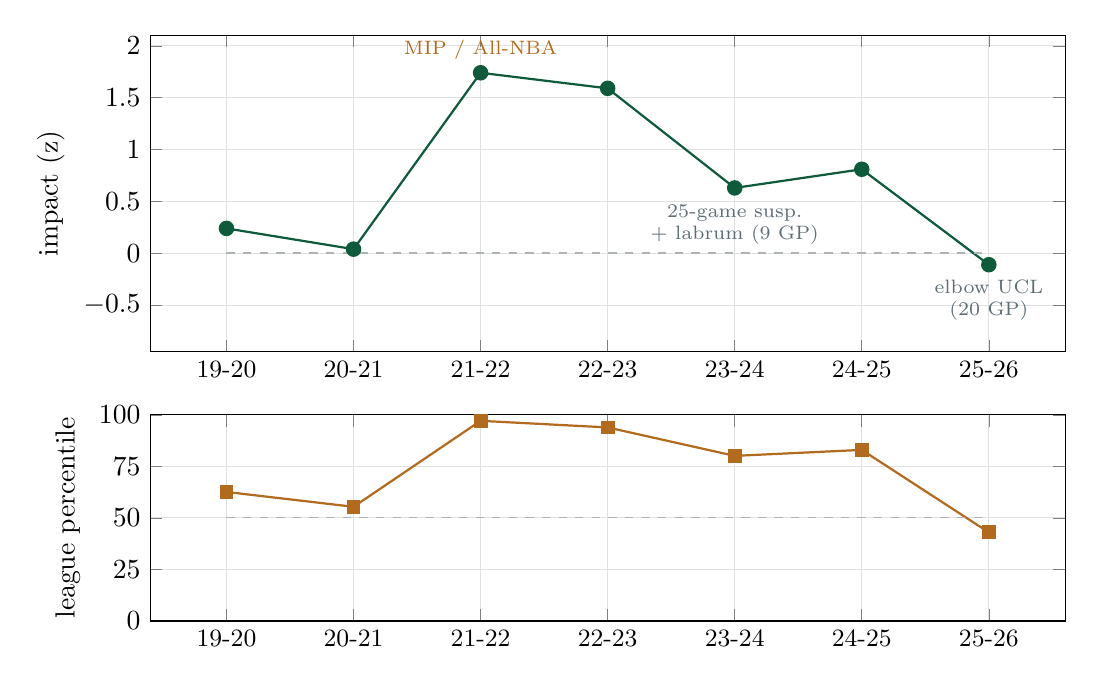
\begin{tikzpicture}
\begin{groupplot}[
  group style={group size=1 by 2, vertical sep=8mm},
  width=13.2cm, xtick=data,
  symbolic x coords={19-20,20-21,21-22,22-23,23-24,24-25,25-26},
  x tick label style={font=\small},
]
\nextgroupplot[height=5.6cm, ylabel={impact (z)},
  ymin=-0.95, ymax=2.1, ytick={-0.5,0,0.5,1,1.5,2},
  grid=major, grid style={fade!40},
  every axis plot/.append style={thick}]
\addplot[color=court, mark=*, mark size=2.4pt] coordinates
  {(19-20,0.24) (20-21,0.04) (21-22,1.74) (22-23,1.59) (23-24,0.63) (24-25,0.81) (25-26,-0.11)};
\addplot[color=fade, dashed, domain=0:6, samples=2] coordinates {(19-20,0) (25-26,0)};
\node[font=\scriptsize, color=amberx, anchor=south] at (axis cs:21-22,1.78) {MIP / All-NBA};
\node[font=\scriptsize, color=steel, anchor=north, align=center] at (axis cs:23-24,0.56)
  {25-game susp.\\ + labrum (9 GP)};
\node[font=\scriptsize, color=steel, anchor=north, align=center] at (axis cs:25-26,-0.16)
  {elbow UCL\\ (20 GP)};
\nextgroupplot[height=4.2cm, ylabel={league percentile}, ymin=0, ymax=100,
  ytick={0,25,50,75,100}, grid=major, grid style={fade!40}]
\addplot[color=amberx, mark=square*, mark size=2.1pt, thick] coordinates
  {(19-20,62.6) (20-21,55.4) (21-22,97.1) (22-23,93.9) (23-24,80.1) (24-25,83.0) (25-26,43.0)};
\addplot[color=fade, dashed] coordinates {(19-20,50) (25-26,50)};
\end{groupplot}
\end{tikzpicture}
\caption{The arc. Top: per-season impact in z units (dashed line = league average).
Bottom: the same thing as a percentile --- in 2021--22 he was better than 97\% of the
league's rotation players; in 2025--26, better than 43\%.}
\label{fig:arc}
\end{figure}

Three things stand out. First, the leap was a \emph{scoring} leap, not a passing one:
from 2020--21 to 2021--22 his volume z jumps $0.77 \to 2.55$, while his creation was
already elite ($\approx +1.9$) as a rookie. Morant didn't learn to create; he learned to
convert volume. Second, the leap held up in the playoffs, where it counts: an
\textbf{8.4 playoff BPM} across two rounds in 2022 (27.1 points, 9.8 rebounds, 8.0
assists per game against Minnesota and Golden State) --- at age 22, one of the strongest
postseason signals any young guard has posted. Third, even at the summit there was a
crack, visible in the Efficiency column: at his career-peak usage in 2022--23 (98th
percentile of the league), his efficiency-for-that-burden was already \emph{negative}
($-0.72$). The engine was extraordinary. The fuel economy never was.

\plainbox{2021--22 Ja was a genuine top-10-caliber season (97th percentile), confirmed in
the playoffs. But even peak Ja scored a lot without scoring \emph{efficiently} --- a flaw
that was survivable at 22 and became the whole story at 26.}

\section{The interruption years, 2023--2025}
\label{sec:interruption}

Then the availability collapsed. Table~\ref{tab:timeline} is the ledger.

\begin{table}[h]
\centering\small
\caption{The absence ledger. Across the three seasons 2023--24 to 2025--26, Morant
appeared in 79 of a possible 246 regular-season games --- 32.1\%. The 2023--24 season
accounts for 73 of the misses: the 25-game suspension first, then a nine-game return,
then 48 games to the shoulder.}
\begin{tabular}{llll}
\toprule
Date & Event & Consequence & Games lost \\
\midrule
Mar 4, 2023 & Firearm on Instagram Live (Denver) & League suspension & 8 \\
May 13, 2023 & Second firearm video & League suspension (start of 23--24) & 25 \\
Jan 2024 & Shoulder labrum tear (practice) & Surgery; season over after 9 GP & 48 \\
Nov 2025 & ``Go ask the coach'' episode & Team suspension & 1 \\
Dec 2025 & Right calf soreness & Two-week absence & $\sim$7 \\
Jan 21, 2026 & Left elbow ligament sprain (vs.\ ATL) & Season over & 33 \\
Jun 29, 2026 & Traded to Portland for Grant \& Murray & --- & --- \\
\bottomrule
\end{tabular}
\label{tab:timeline}
\end{table}

Two details in this stretch resist the standard telling. His nine-game 2023--24 cameo was
\emph{good} (25.1 points, 8.1 assists per game, 80th-percentile impact) before the
shoulder ended it. And 2024--25, the forgotten season, was genuinely solid: over 1{,}519
minutes he graded at the 83rd percentile --- roughly a top-50 player when on the floor
--- with a 94th-percentile foul-drawing rate. Morant did not slide gently for three
years. He was a clearly good player right up until 2025--26, and then he fell off a
ledge in one season.

\section{The collapse season, 2025--26: three answers}
\label{sec:collapse}

Twenty games, 569 minutes: 19.5 points on .410 shooting, 8.1 assists, and the worst
efficiency of his life. The season ended January 21 with an elbow ligament sprain, two
games after he returned from a calf absence. We ask three questions of it.

\subsection{Question 1: did his whole game collapse?}

No --- and this is the strangest fact in the paper. Compare the last two rows of
Table~\ref{tab:zmatrix}, drawn in Figure~\ref{fig:dumbbell}. Every efficiency-linked
number cratered to career-worst levels. And at the same time his \textbf{creation
($+3.19$) and offensive load ($+2.90$) hit career highs} --- his assist rate (44.7\%) was
a 96th-percentile figure. The player in those 20 games was a career-best distributor
carrying a career-peak burden who could not put the ball in the basket. That
combination --- process intact, outcomes broken --- is what a cold streak looks like.
Twenty games cannot prove that reading; what they can do is fail to match the
alternative, because eroded athletes do not usually set career highs in the two most
demanding process stats while their shots rim out.

\begin{figure}[h]
\centering
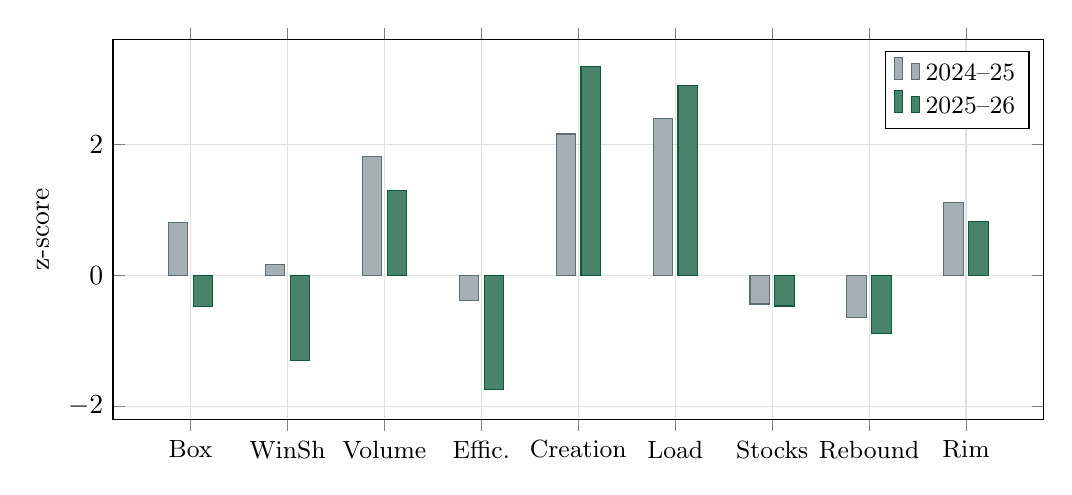
\begin{tikzpicture}
\begin{axis}[
  width=13.4cm, height=6.4cm, ybar, bar width=7pt,
  symbolic x coords={Box,WinSh,Volume,Effic.,Creation,Load,Stocks,Rebound,Rim},
  xtick=data, ymin=-2.2, ymax=3.6, ylabel={z-score},
  grid=major, grid style={fade!40},
  legend style={font=\small, at={(0.985,0.97)}, anchor=north east},
  x tick label style={font=\small},
]
\addplot[fill=steel!55, draw=steel] coordinates
  {(Box,0.80) (WinSh,0.17) (Volume,1.81) (Effic.,-0.38) (Creation,2.16)
   (Load,2.39) (Stocks,-0.44) (Rebound,-0.65) (Rim,1.11)};
\addplot[fill=court!75, draw=court] coordinates
  {(Box,-0.48) (WinSh,-1.31) (Volume,1.30) (Effic.,-1.75) (Creation,3.19)
   (Load,2.90) (Stocks,-0.47) (Rebound,-0.89) (Rim,0.82)};
\legend{2024--25, 2025--26}
\end{axis}
\end{tikzpicture}
\caption{The paradox season. Green bars (2025--26) vs.\ grey (2024--25): the two tallest
green bars --- creation and load --- are career highs; the efficiency bars are career lows.}
\label{fig:dumbbell}
\end{figure}

\subsection{Question 2: bad shots, or missed shots?}
\label{sec:mixmake}

The visible symptom was an ugly shot diet: 46\% of his attempts from mid-range, long twos
tripling. Everyone blamed the shot selection. The accounting disagrees. Using \ctg{} zone
data (where shots came from, and how often they went in), the change in effective
field-goal percentage between 2024--25 and 2025--26 splits \emph{exactly} into a
shot-selection part and a shot-making part:
\begin{equation}
\Delta \mathrm{eFG}
= \underbrace{\textstyle\sum_z (f'_z - f_z)\, \bar{a}_z\, w_z}_{\text{selection (where)}}
\;+\;
\underbrace{\textstyle\sum_z \bar{f}_z\, (a'_z - a_z)\, w_z}_{\text{making (whether)}},
\label{eq:shapley}
\end{equation}
where $f_z$ is the share of shots from zone $z$, $a_z$ the accuracy there, and threes get
their extra 50\% credit ($w_z$). The split is symmetric --- neither part is favored.

\begin{table}[h]
\centering\small
\caption{Where vs.\ whether, 2024--25 $\to$ 2025--26. His eFG fell about 5.7 points;
selection explains 0.7 of them.}
\begin{tabular}{lccccc|c}
\toprule
 & Rim & Short mid & Long mid & Corner 3 & Non-corner 3 & eFG \\
\midrule
Share of shots (24--25) & 33\% & 35\% & 4\% & 6\% & 21\% & \multirow{2}{*}{.510} \\
Accuracy (24--25) & 62\% & 45\% & 39\% & 35\% & 32\% & \\
\midrule
Share of shots (25--26) & 30\% & 37\% & 9\% & 4\% & 20\% & \multirow{2}{*}{.453} \\
Accuracy (25--26) & 61\% & 40\% & 39\% & 50\% & 19\% & \\
\midrule
\multicolumn{6}{l}{Total drop $= -5.7$ pts $=$ selection $\mathbf{-0.7}$ $+$ making $\mathbf{-5.0}$} & \\
\multicolumn{6}{l}{If he'd kept the \emph{old diet} at the new accuracy: eFG $= .462$ (barely helps)} & \\
\multicolumn{6}{l}{If he'd hit the \emph{new diet} at the old accuracy: eFG $= .505$ (nearly normal)} & \\
\bottomrule
\end{tabular}
\label{tab:mixmake}
\end{table}

\textbf{At the zone level, 88\% of the collapse was missing, not choosing.} Had he
converted his ugly new shot diet at his normal rates, his efficiency would have been
almost fine (.505). Fixing the diet without fixing the makes recovers almost nothing
(.462). The shot chart looked broken because the shots missed, not mainly because of
where they were taken.

One honest limitation. ``Selection'' here means \emph{zone mix} --- the five \ctg{}
zones --- because that is what the decomposition can see. It cannot see defender
distance, pull-up versus catch-and-shoot, shot-clock pressure, or how contested the
attempts were; two non-corner threes can differ enormously in difficulty. If his
2025--26 attempts were systematically harder \emph{within} zones, some of the
``missing'' is really hidden shot selection. The defensible reading is therefore: the
collapse was not primarily about \emph{where} he shot. How much of the conversion drop
was shot difficulty rather than pure misses, zone data cannot separate --- which is one
more reason the sample-size analysis of the next section matters.

\subsection{Question 3: is the missing even real?}
\label{sec:ci}

Missing, then --- over what sample? A 95\% confidence interval answers the question every
hot take skips: \emph{given this few attempts, where could his true shooting level
plausibly be?} (Formally we use Wilson score intervals; the formula is
Appendix~\ref{app:spec}, eq.~\ref{eq:wilson}.)

\begin{table}[h]
\centering\small
\caption{2025--26 shooting splits with 95\% confidence bands. Read the last column: only
one split moved beyond doubt, and it moved \emph{up}.}
\begin{tabular}{lccccl}
\toprule
Split & Made/Att & Season & Plausible range & Career & Verdict \\
\midrule
3P\% & 20/85 & .235 & [.158, .336] & $\approx$.315 & career norm inside the band \\
FG\% & 132/322 & .410 & [.358, .464] & $\approx$.465 & borderline \\
Rim FG\% & 48/73 & .658 & [.544, .756] & $\approx$.62 & fully consistent \\
FT\% & 105/117 & .897 & [.829, .940] & .776 & \textbf{significantly better} \\
\bottomrule
\end{tabular}
\label{tab:wilson}
\end{table}

\begin{figure}[h]
\centering
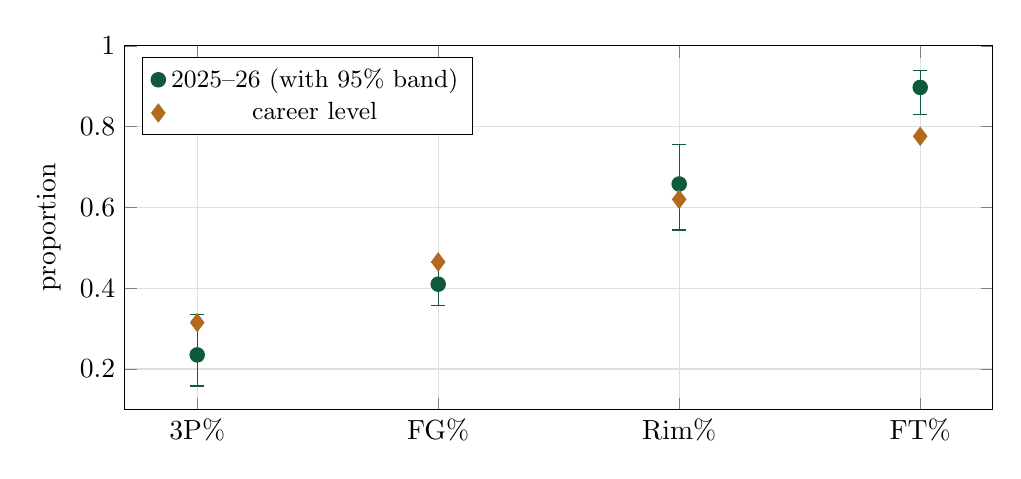
\begin{tikzpicture}
\begin{axis}[
  width=12.6cm, height=6.2cm,
  symbolic x coords={3P\%, FG\%, Rim\%, FT\%},
  xtick=data, ymin=0.1, ymax=1.0, ylabel={proportion},
  grid=major, grid style={fade!40},
  legend style={font=\small, at={(0.02,0.97)}, anchor=north west},
]
\addplot[only marks, mark=*, court, mark options={fill=court}, mark size=2.6pt,
  error bars/.cd, y dir=both, y explicit]
  coordinates {
    (3P\%,0.235) += (0,0.101) -= (0,0.077)
    (FG\%,0.410) += (0,0.054) -= (0,0.052)
    (Rim\%,0.658) += (0,0.098) -= (0,0.114)
    (FT\%,0.897) += (0,0.043) -= (0,0.068)
  };
\addplot[only marks, mark=diamond*, amberx, mark options={fill=amberx}, mark size=3.2pt] coordinates
  {(3P\%,0.315) (FG\%,0.465) (Rim\%,0.62) (FT\%,0.776)};
\legend{2025--26 (with 95\% band), career level}
\end{axis}
\end{tikzpicture}
\caption{The sample-size problem, drawn. Green dots: 2025--26, with the range his true
level could plausibly occupy. Amber diamonds: career levels. Three of four bands contain
his career level. The one clear change is the free throw --- upward.}
\label{fig:ci}
\end{figure}

The three-point collapse --- the number most responsible for the ``he's done'' narrative
--- rests on 85 attempts, and its band comfortably contains his career norm. To be
precise about what that means: the sample cannot confidently distinguish a genuine
decline from ordinary shooting variance. It does not prove the miss was a cold streak;
it proves nobody can yet prove it wasn't. Meanwhile the free throw, the purest touch
test in basketball, improved so much the band excludes his career average from
\emph{below}. That is strong evidence against a broad loss of shooting touch --- though
not against every physical story, since a player can lose lift or separation on live-play
jumpers while improving from a standstill. The simplest versions of ``his shot is
gone,'' however, predict the opposite of what happened at the stripe.

\plainbox{Three answers: (1) his playmaking hit a career high while the shooting failed;
(2) at the zone level, the failure was 88\% missing, 12\% shot selection; (3) at 85
threes, the sample can't tell genuine decline from an ordinary cold streak --- and his
free-throw touch got \emph{better}. The one caveat that is real: his rim-attack rate has
been sliding for seven years (Figure~\ref{fig:diet}).}

\subsection{The seven-season shot profile}

Career context, and the one concession the optimistic reading must make. His rim
frequency has eroded steadily since the rookie peak --- from 49\% of attempts to 30\%
(Figure~\ref{fig:diet}) --- a real, slow trend consistent with age and injury. But the
accuracy panel (Figure~\ref{fig:acc}) shows what actually distinguished the collapse
year: the three-ball fell out of its seven-year band, on the smallest sample, while rim
conversion held steady and the free throw kept climbing.

\begin{figure}[h]
\centering
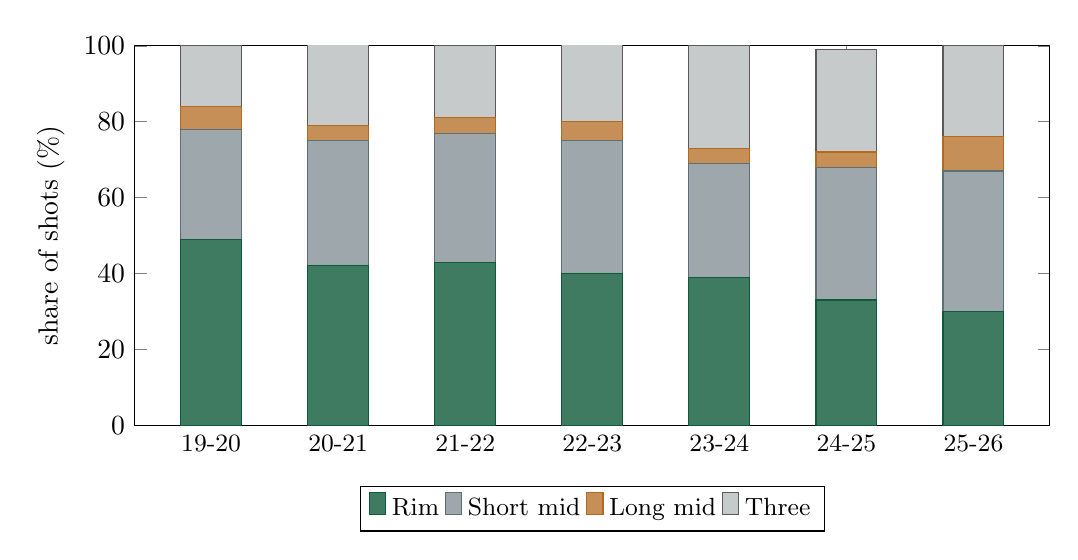
\begin{tikzpicture}
\begin{axis}[
  width=13.2cm, height=6.4cm, ybar stacked, bar width=22pt,
  symbolic x coords={19-20,20-21,21-22,22-23,23-24,24-25,25-26},
  xtick=data, ymin=0, ymax=100, ylabel={share of shots (\%)},
  legend style={font=\small, at={(0.5,-0.16)}, anchor=north, legend columns=4},
  x tick label style={font=\small},
]
\addplot[fill=court!80, draw=court] coordinates
  {(19-20,49) (20-21,42) (21-22,43) (22-23,40) (23-24,39) (24-25,33) (25-26,30)};
\addplot[fill=steel!60, draw=steel] coordinates
  {(19-20,29) (20-21,33) (21-22,34) (22-23,35) (23-24,30) (24-25,35) (25-26,37)};
\addplot[fill=amberx!75, draw=amberx] coordinates
  {(19-20,6) (20-21,4) (21-22,4) (22-23,5) (23-24,4) (24-25,4) (25-26,9)};
\addplot[fill=fade!70, draw=fade!50!black] coordinates
  {(19-20,16) (20-21,22) (21-22,19) (22-23,21) (23-24,27) (24-25,27) (25-26,24)};
\legend{Rim, Short mid, Long mid, Three}
\end{axis}
\end{tikzpicture}
\caption{Where his shots come from, by season. The green (rim) share halves across seven
years --- the one long-run decline in the data that is unambiguously real.}
\label{fig:diet}
\end{figure}

\begin{figure}[h]
\centering
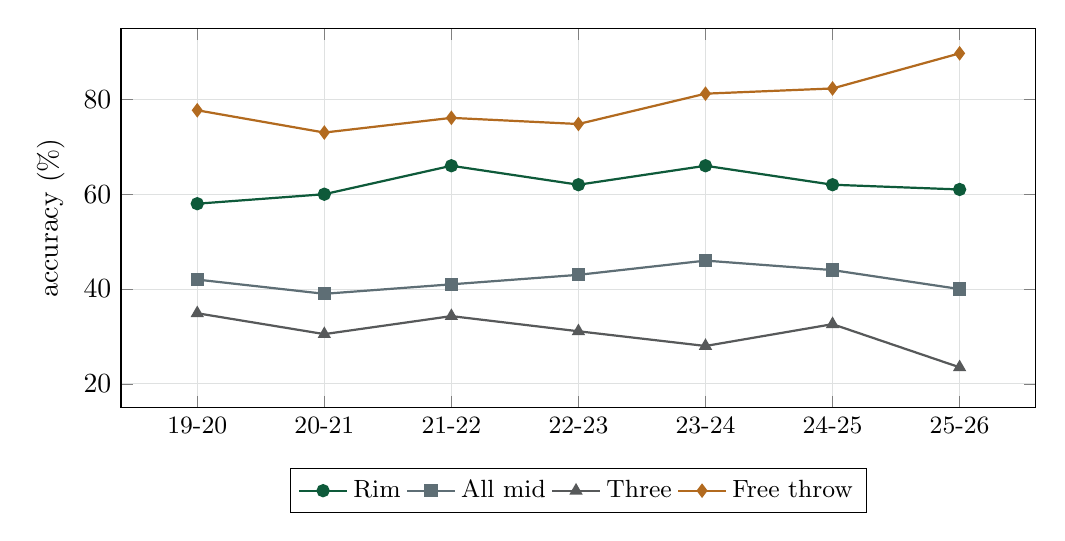
\begin{tikzpicture}
\begin{axis}[
  width=13.2cm, height=6.4cm,
  symbolic x coords={19-20,20-21,21-22,22-23,23-24,24-25,25-26},
  xtick=data, ymin=15, ymax=95, ylabel={accuracy (\%)},
  grid=major, grid style={fade!40},
  legend style={font=\small, at={(0.5,-0.16)}, anchor=north, legend columns=4},
  x tick label style={font=\small},
  every axis plot/.append style={thick, mark size=2pt},
]
\addplot[color=court, mark=*] coordinates
  {(19-20,58) (20-21,60) (21-22,66) (22-23,62) (23-24,66) (24-25,62) (25-26,61)};
\addplot[color=steel, mark=square*] coordinates
  {(19-20,42) (20-21,39) (21-22,41) (22-23,43) (23-24,46) (24-25,44) (25-26,40)};
\addplot[color=fade!50!black, mark=triangle*] coordinates
  {(19-20,34.9) (20-21,30.5) (21-22,34.3) (22-23,31.1) (23-24,28.0) (24-25,32.6) (25-26,23.5)};
\addplot[color=amberx, mark=diamond*] coordinates
  {(19-20,77.7) (20-21,73.0) (21-22,76.1) (22-23,74.8) (23-24,81.2) (24-25,82.3) (25-26,89.7)};
\legend{Rim, All mid, Three, Free throw}
\end{axis}
\end{tikzpicture}
\caption{Whether they go in, by season. Rim conversion (green) holds a seven-year band;
the free throw (amber) climbs to .897; the three (grey) crashes --- on 85 attempts. The two
purest touch measures moving in opposite directions is the season's central oddity, and
randomness is its cheapest explanation.}
\label{fig:acc}
\end{figure}

\section{How \#140 happens}
\label{sec:value}

Table~\ref{tab:pipeline} runs Morant through the full \gravity{} pipeline, step by step
(equation numbers refer to Appendix~\ref{app:spec}). Notice what the arithmetic does and
doesn't say. His blended two-season rate ($+0.30$) still describes an above-average NBA
player. What produces \#140 is the reliability stack: availability $0.896$ (29 weighted
games against a 55-game standard), role $0.958$, injury override $0.950$ --- multiplying
to $0.815$ of his value above replacement. \gravity{} prices Morant like an asset with a
high expected return and terrible delivery risk. Four days after the ranking date, an
actual front office priced him identically, trading him for two salary-matching forwards.
Because several steps in the pipeline are judgment calls --- the override, the anchor,
the season weights --- Appendix~\ref{app:sens} re-runs the entire ranking under
alternative choices and reports how much \#140 moves.

\begin{table}[h]
\centering\small
\caption{The \gravity{} pipeline for Morant, July 2026, every step shown.}
\begin{tabular}{llr}
\toprule
Step & Quantity & Value \\
\midrule
Impact, 2025--26 [eq.~\ref{eq:impact}] & 569 minutes, on/off $+1.5$ & $-0.094$ \\
Impact, 2024--25 [eq.~\ref{eq:impact}] & 1519 minutes & $+0.751$ \\
Blend weight [eq.~\ref{eq:blend}] & recent season counts $0.75\times$ per minute & $0.529$ \\
Blended rate & $0.529(-0.094) + 0.471(0.751)$ & $+0.304$ \\
Small-sample shrink [eq.~\ref{eq:cred}] & $c=\sqrt{2088/2200}$ toward replacement & $+0.248$ \\
Playoff / age terms & --- & $0,\ 0$ \\
Availability [eq.~\ref{eq:avail}] & 29 weighted games of 55 & $\times\,0.896$ \\
Role size [eq.~\ref{eq:role}] & 28.4 min/game & $\times\,0.958$ \\
Injury override [eq.~\ref{eq:inj}] & elbow ligament, season-ending & $\times\,0.950$ \\
Final z & $-1.9 + (0.248+1.9)(0.815)$ & $-0.149$ \\
\midrule
\textbf{\gravity{} score} & $50 + 15(-0.149)$ & $\mathbf{47.8}$ \\
\textbf{Rank} & of 644 (all veterans + 2026 draft class) & \textbf{\#140} \\
\bottomrule
\end{tabular}
\label{tab:pipeline}
\end{table}

\section{What Portland is getting: the price of every future}
\label{sec:prognosis}

Morant enters 2026--27 at 27, sharing a backcourt with Damian Lillard (36, returning
from an Achilles rupture), on a roster that just made the playoffs without either of
them. His future has two separate uncertainties --- \emph{how well he plays} and
\emph{how often he plays} --- and bundling them into named scenarios hides the trade.
So Table~\ref{tab:matrix} prices them separately: each cell runs the full pipeline
(blend with the 569-minute 2025--26 season, credibility shrink, availability and role
multipliers) for an assumed 2026--27 per-minute impact and games total, at 31 minutes
per game with no injury override assumed. These are \emph{illustrative prices, not
probabilities}: the framework says what each future is worth, not which one arrives.

\begin{table}[h]
\centering\small
\caption{The availability $\times$ impact matrix. Cell = projected July 2027 score
(equivalent rank in the July 2026 edition). Row levels are his own career benchmarks:
$-0.10$ is the 2025--26 collapse, $+0.80$ is 2024--25, $+1.65$ is the 2021--23 peak.}
\begin{tabular}{lccc}
\toprule
2026--27 per-minute level & 25 GP & 50 GP & 65 GP \\
\midrule
$-0.10$ (repeat collapse)   & 39.7 {\scriptsize(\#281)} & 46.2 {\scriptsize(\#166)} & 47.8 {\scriptsize(\#138)} \\
$+0.80$ (2024--25 level)    & 47.1 {\scriptsize(\#154)} & 57.2 {\scriptsize(\#53)}  & 59.8 {\scriptsize(\#35)}  \\
$+1.65$ (2021--23 peak)     & 54.0 {\scriptsize(\#77)}  & 67.6 {\scriptsize(\#10)}  & 71.2 {\scriptsize(\#7)}   \\
\bottomrule
\end{tabular}
\label{tab:matrix}
\end{table}

The matrix makes three facts legible that the bundled scenarios obscured. First, the
corner cells agree on a striking symmetry: playing at his 2024--25 level for only 25
games (47.1) is worth almost exactly the same as playing a full healthy season at his
collapse level (47.8) --- and the latter is his current score. Health and form are
near-perfect substitutes at the bottom of the table. Second, the big jumps live in the
\emph{games} direction: at the 2024--25 level, going from 25 to 50 games buys +10.1
points; going from the 2024--25 level to the peak level at fixed 50 games buys +10.4.
Portland's return on a healthy Morant is as large as its return on a resurgent one.
Third, top-50 requires \emph{both}: no 25-game column reaches it, and no collapse-level
row does.

Which cells deserve weight is a judgment the reader can make with the paper's evidence:
the skills that collapse first in genuinely declining guards --- rim conversion, foul
drawing, free-throw touch --- are respectively stable, elite (seven straight seasons at
the 86th percentile or better), and improving, while the stats that cratered are the
ones a confidence interval refuses to certify. That argues against loading the bottom
row. Against it stand the two real risks: a rim-attack rate that has halved in seven
years, and the availability record of Table~\ref{tab:timeline}. The binding constraint
on Ja Morant has never been a shooting slump. It is that since 2023 he has played
32.1\% of his team's games. \gravity{} will believe the rise again when the denominator
does.

\section{Conclusion}

Measured with one instrument across seven seasons, Morant's career is a steep genuine
rise ($+1.7\sigma$, twice), an availability catastrophe, and one 569-minute season the
data cannot fully judge. Most of the observed efficiency decline came from worse
conversion rather than from where he shot --- though the sample is too small to say how
much of that conversion drop is lasting decline rather than variance. What the data can
certify: his creation set a career high, his rim conversion held, his free-throw touch
improved; against that, his rim-attack rate has fallen for seven straight years and his
availability record is severe. \#140 of 644 is a defensible price for that bundle of
uncertainty --- robust, per Appendix~\ref{app:sens}, to every judgment call we could
vary --- and it should not be read as a claim that 139 players possess more healthy,
on-court talent. It is the right price for the risk, and probably the wrong forecast of
the talent. Both statements are the same mathematics, read in two directions.

\section*{Revision note (v2, July 11, 2026)}
Following a detailed external review, this version corrects two accounting errors and
tightens several claims. (1) The absence ledger charged 73 games to the January 2024
shoulder injury; the correct figure is 48, since the 25-game suspension --- listed on
its own row --- and the nine games he played account for the rest of that season.
(2) The three-season availability denominator was stated as 249 games (31.7\%); the
correct figures are 246 and 32.1\%. (3) The Shapley decomposition is now explicitly
scoped to zone-level selection; the free-throw and cold-streak inferences are stated
with the caveats the intervals actually support; the three bundled forward scenarios
were replaced by the availability~$\times$~impact matrix of Table~\ref{tab:matrix},
recomputed under a single stated convention; and Appendix~\ref{app:sens} (model
sensitivity) was added. The errors were ours. Nothing in the correction changes the
ranking itself, which is computed from the data, not from the prose.

\appendix
\section{The full GRAVITY specification}
\label{app:spec}

For completeness; nothing in the body requires this section. Let season $y$ have player
set $\mathcal{P}_y$ with minutes $m_i$. For any statistic $x_k(i)$, minutes-weighted
moments and clipped z-scores are
\begin{equation}
\mu_k = \frac{\sum_i m_i x_k(i)}{\sum_i m_i}, \quad
\sigma_k = \Bigl(\tfrac{\sum_i m_i (x_k(i)-\mu_k)^2}{\sum_i m_i}\Bigr)^{1/2}, \quad
z_k(i) = \mathrm{clip}\bigl((x_k(i)-\mu_k)/\sigma_k,\ \pm 4\bigr).
\label{eq:moments}
\end{equation}
Component constructions:
\begin{align}
\text{eff}(i) &= (\mathrm{TS}_i - \mu_{\mathrm{TS}})\cdot 100 \cdot
(\mathrm{clip}(\mathrm{USG}_i, 8, 36)/20)^{0.7}, \\
\text{creation}(i) &= \mathrm{AST\%}_i - 0.55\,\mathrm{TOV\%}_i, \qquad
\text{load}(i) = \mathrm{USG}_i + 0.4\,\mathrm{AST\%}_i, \\
\text{stocks}(i) &= 2\,\mathrm{STL\%}_i + 1.2\,\mathrm{BLK\%}_i, \qquad
\text{rim}(i) = 100\,\mathrm{FTr}_i + 200\cdot\text{dunk share}_i.
\end{align}
Skill blend (current season): $S = 0.27 z_{\text{vol}} + 0.19 z_{\text{eff}} + 0.22
z_{\text{crea}} + 0.09 z_{\text{load}} + 0.10 z_{\text{stk}} + 0.05 z_{\text{reb}} +
0.08 z_{\text{rim}}$. Season impact, with \ctg{} filtered on/off regressed by minutes and
a within-season small-sample shrink:
\begin{equation}
I_y(i) = \Bigl[0.44 z_{\mathrm{BPM}} + 0.12 z_{\mathrm{WS/48}}
+ 0.14\, z\bigl(\Delta_{\text{on/off}} \min(1, m_i/2400)\bigr) + 0.30\, S\Bigr]
\sqrt{\min(1, m_i/800)}.
\label{eq:impact}
\end{equation}
Two-year blend and credibility shrink toward replacement $\rho = -1.9$:
\begin{equation}
w = \frac{0.75 m_y}{0.75 m_y + 0.25 m_{y-1}}, \qquad
R = w I_y + (1{-}w) I_{y-1},
\label{eq:blend}
\end{equation}
\begin{equation}
\tilde{R} = cR + (1{-}c)\rho, \qquad c = \sqrt{\tfrac{\min(m_y + m_{y-1},\, 2200)}{2200}}.
\label{eq:cred}
\end{equation}
Playoff evidence $\pi = \mathrm{clip}(0.12(\mathrm{BPM}^{po}{-}\mathrm{BPM}^{rs})
\min(1, m^{po}/300)/2.6, \pm 0.30)$; age nudge $\alpha$ ($+0.055$/yr under 24,
$-0.045$/yr past 30, clipped $[-0.30, 0.25]$). Reliability multipliers:
\begin{align}
A &= 0.78 + 0.22 \min\bigl(1, (0.7 g_y + 0.3 g_{y-1})/55\bigr), \label{eq:avail}\\
\Phi &= 0.62 + 0.38 \min\bigl(1, \max(\mathrm{mpg}_y, 0.85\,\mathrm{mpg}_{y-1})/32\bigr), \label{eq:role}\\
J &\in [0.78, 1.00] \text{ (documented injury override).} \label{eq:inj}
\end{align}
Final score: $G = 50 + 15[\rho + (\tilde{R} + \pi + \alpha - \rho) A \Phi J]$. The
historical variant \gravity-RS used for Table~\ref{tab:zmatrix} deletes the on/off term
(not uniformly available pre-2024) and renormalizes: $I^{RS} = [0.533 z_{\mathrm{BPM}} +
0.133 z_{\mathrm{WS/48}} + 0.333 S']\sqrt{\min(1, m/800)}$, with $S'$ using prior-season
skill weights and a free-throw-rate-only rim term. Wilson 95\% intervals used in
Section~\ref{sec:ci}:
\begin{equation}
p \in \Bigl(\hat{p} + \tfrac{z^2}{2n} \pm z\sqrt{\tfrac{\hat{p}(1-\hat{p})}{n}
+ \tfrac{z^2}{4n^2}}\Bigr)\Big/\bigl(1 + z^2/n\bigr), \qquad z = 1.96.
\label{eq:wilson}
\end{equation}

\subsection*{Data}
Basketball-Reference league, player and playoff tables (2019--20 to 2025--26);
Cleaning the Glass subscriber database (filtered on/off, shot zones, foul drawing),
accessed July 10, 2026; Sports-Reference CBB. The specification is identical to the
July 10, 2026 ``The 644'' ranking (v3), in which Morant's pipeline values appear
verbatim. No external rankings or projections were consulted.

\section{How much do the model's choices matter?}
\label{app:sens}

A transparent model is not the same thing as a validated one. The weights in
Appendix~\ref{app:spec} --- and the replacement anchor, the availability standard, and
the injury overrides --- were specified by judgment before any player was ranked; they
were not fitted to a target variable. Publishing them makes the judgment inspectable.
It does not make it correct. The honest next question is: how much does this paper's
conclusion depend on those choices?

Table~\ref{tab:sens} answers it by re-running the \emph{entire} 644-player pipeline ---
rookies included, since their scores are percentiles of the veteran distribution ---
under each variation, and reporting where Morant lands. Each row changes exactly one
thing.

\begin{table}[h]
\centering\small
\caption{Sensitivity of Morant's July 2026 placement. Every variation re-ranks all 644
players; rank is within that variation's own ranking.}
\begin{tabular}{lcc}
\toprule
Model variation & Score & Rank \\
\midrule
Baseline \gravity{} v3, as published & 47.8 & \#140 \\
Injury overrides removed entirely (all $J{=}1$) & 49.1 & \#130 \\
Equal two-season weights ($0.50/0.50$ vs.\ $0.75/0.25$) & 50.3 & \#112 \\
Availability standard 65 games (vs.\ 55) & 47.2 & \#147 \\
Alternate impact weights (BPM $.35$, WS/48 $.15$, on/off $.20$) & 47.5 & \#147 \\
Replacement level $-1.6$ (vs.\ $-1.9$) & 48.7 & \#138 \\
Reliability stack removed ($A{=}\Phi{=}J{=}1$; per-minute talent only) & 53.7 & \#112 \\
\bottomrule
\end{tabular}
\label{tab:sens}
\end{table}

Every variation lands him between \#112 and \#147. The two that move him most ---
equal season weights, and deleting the reliability machinery altogether --- are both
versions of the same question, \emph{how much should the solid 2024--25 season count?},
and both answer \#112: even the reading most generous to his track record does not put
him inside the top 100 on this data. In the other direction, no tightening we tested
pushes him past \#147. The paper's headline number is not an artifact of any single
judgment call; within this family of specifications, ``a clearly good player, heavily
discounted for delivery risk'' is the only available conclusion.

What this appendix cannot do is validate the model against the future --- that is what
the Forecast Ledger is for. \gravity{}'s registered predictions are graded in public,
annually, starting with the July 2027 Forecast Audit; predictive validation accrues
there, one scored forecast at a time.

\begin{thebibliography}{9}
\bibitem{bbref} Basketball-Reference.com, league and player tables, accessed July 10, 2026.
\bibitem{ctg} Cleaning the Glass, player on/off and shooting tables (subscription),
accessed July 10, 2026. \url{https://cleaningtheglass.com/stats/player/4573}
\bibitem{srcbb} Sports-Reference College Basketball, Temetrius ``Ja'' Morant player page.
\bibitem{elbow} ``Grizzlies rule Ja Morant out for rest of season due to elbow sprain,''
Yahoo Sports / NBA.com news, February 2026.
\bibitem{susp} ``Why was Ja Morant suspended? What we know about the latest Grizzlies
drama,'' ESPN.com, November 2025.
\bibitem{susp23} NBA Communications, 25-game suspension announcement, June 16, 2023.
\bibitem{trade} ESPN.com 2026 offseason trade tracker: Grizzlies trade Morant to Trail
Blazers for Jerami Grant and Kris Murray, June 29, 2026.
\end{thebibliography}

\end{document}
